\section{Mode Operasi Block Cipher}

Block cipher mengenkripsi satu blok. Untuk data lebih panjang, digunakan \textbf{mode operasi}. Mode operasi sangat penting karena menentukan bagaimana block cipher digunakan untuk mengenkripsi data yang lebih panjang dari satu blok, serta mempengaruhi keamanan dan efisiensi implementasi.

Mode operasi block cipher berevolusi dari waktu ke waktu untuk mengatasi berbagai kelemahan keamanan. Menurut Wikipedia, mode-mode paling awal seperti ECB, CBC, OFB, dan CFB telah ada sejak tahun 1981 dan distandarisasi dalam FIPS 81. Seiring waktu, mode baru seperti CTR dan GCM dikembangkan untuk mengatasi kelemahan mode-mode sebelumnya dan menyediakan fitur tambahan seperti autentikasi.

\subsection{ECB (Electronic Codebook)}

Setiap blok dienkripsi independen. \textbf{Kelemahan}: Blok plaintext identik menghasilkan ciphertext identik—rentan analisis pola. Tidak direkomendasikan untuk data sensitif. Menurut Wikipedia, ECB adalah mode yang paling sederhana tetapi juga paling tidak aman karena tidak menyediakan semantic security dan sangat rentan terhadap serangan pattern analysis.

ECB memiliki kelemahan fundamental yang sangat serius dalam aplikasi praktis. Menurut sumber keamanan, ECB tidak menyediakan semantic security karena plaintext identik menghasilkan ciphertext identik, yang sangat berbahaya untuk data terstruktur seperti gambar atau dokumen terformat. Mode ini hanya cocok untuk enkripsi data acak yang sangat pendek atau sebagai komponen dalam protokol yang lebih kompleks.

\subsection{CBC (Cipher Block Chaining)}

Setiap blok plaintext di-XOR dengan ciphertext blok sebelumnya sebelum enkripsi. Blok pertama di-XOR dengan \textbf{IV} (Initialization Vector). IV harus acak dan unik per enkripsi, dapat dikirim bersama ciphertext. Menurut Wikipedia, CBC adalah mode yang paling umum digunakan sebelum munculnya mode AEAD modern.

CBC menyediakan keamanan yang jauh lebih baik dibandingkan ECB karena setiap blok ciphertext bergantung pada semua blok sebelumnya. Menurut sumber keamanan, IV harus unik untuk setiap enkripsi dengan kunci yang sama untuk mencegah serangan replay dan memastikan semantic security. Namun, CBC tidak dapat diparalelkan selama enkripsi dan rentan terhadap padding oracle attacks.

\subsection{Padding (PKCS\#7)}

Jika panjang plaintext tidak kelipatan ukuran blok, digunakan padding. PKCS\#7 menambah $k$ byte bernilai $k$ (1--block size) \cite{rfc5652}:
\begin{itemize}
  \item Jika blok sisa 5 byte pada AES (16 byte), tambahkan 11 byte bernilai 0x0B.
  \item Jika plaintext tepat kelipatan blok, tambahkan satu blok penuh bernilai 0x10.
\end{itemize}

Padding PKCS\#7 adalah standar industri yang digunakan secara luas dalam implementasi CBC dan mode-mode lainnya. Menurut RFC 5652, padding ini dirancang untuk dapat dihapus secara unik setelah dekripsi, mencegah ambiguitas dalam menentukan panjang plaintext asli. Namun, implementasi padding yang salah dapat menyebabkan kerentanan padding oracle attacks yang sangat serius.

\begin{catatan}
Pada CBC, padding yang salah dapat memicu \textit{padding oracle} jika pesan kesalahan dibedakan. Gunakan mode AEAD (mis. GCM) untuk integritas \cite{nist800_38d}.
\end{catatan}

\subsection{CFB dan OFB}

CFB (Cipher Feedback) dan OFB (Output Feedback): mengubah block cipher menjadi stream cipher. Keduanya membutuhkan IV. Menurut Wikipedia, CFB dan OFB dikembangkan untuk mengatasi keterbatasan ECB dan CBC, terutama untuk aplikasi yang memerlukan stream cipher atau komunikasi real-time.

CFB dan OFB memiliki karakteristik yang berbeda yang membuatnya cocok untuk aplikasi tertentu. Menurut sumber keamanan, CFB memungkinkan enkripsi data yang tidak kelipatan blok dan dapat pulih dari error bit, sedangkan OFB memberikan stream cipher yang sinkron dan lebih resisten terhadap error propagation. Keduanya memerlukan IV yang unik untuk setiap sesi komunikasi.

\subsection{CTR (Counter Mode)}

CTR membuat \textit{keystream} dengan mengenkripsi nonce||counter, lalu di-XOR dengan plaintext. Mode ini paralel dan tidak memerlukan padding \cite{nist800_38a}. Menurut Wikipedia, CTR menjadi sangat populer karena efisiensinya dan kemampuan untuk diparalelkan, membuatnya ideal untuk implementasi modern pada multi-core processors.

CTR menawarkan keuntungan performa yang signifikan dibandingkan mode-mode lainnya. Menurut sumber keamanan, CTR dapat diimplementasikan secara paralel penuh baik untuk enkripsi maupun dekripsi, dan tidak memerlukan padding karena keystream dapat dipotong sesuai panjang plaintext. Namun, nonce harus unik untuk setiap enkripsi dengan kunci yang sama untuk mencegah keystream reuse.

\subsection{AEAD: GCM/CCM}

GCM dan CCM memberikan kerahasiaan sekaligus integritas (AEAD). Nonce harus unik; reuse nonce pada GCM dapat membocorkan kunci \cite{nist800_38d}. Menurut Wikipedia, AEAD mode menjadi standar modern karena menyederhanakan implementasi keamanan dengan menggabungkan enkripsi dan autentikasi dalam satu operasi atomik.

GCM (Galois/Counter Mode) dan CCM (Counter with CBC-MAC) mewakili evolusi terbaru dalam mode operasi block cipher. Menurut sumber keamanan, GCM menggunakan Galois Field multiplication untuk autentikasi yang sangat efisien dalam perangkat keras, sedangkan CCM menggabungkan CTR untuk enkripsi dengan CBC-MAC untuk autentikasi. Keduanya menyediakan keamanan yang komprehensif dengan overhead minimal.

\subsection{XTS untuk Storage}

XTS dirancang untuk enkripsi disk/penyimpanan, menghindari pola blok berulang pada sektor \cite{nist800_38e}. Menurut Wikipedia, XTS dikembangkan khusus untuk aplikasi penyimpanan data di mana data dapat diubah secara parsial dan memerlukan tweakable encryption untuk mencegah pola yang dapat dieksploitasi.

XTS menggunakan tweakable encryption yang memungkinkan modifikasi data tanpa mengenkripsi ulang seluruh sektor. Menurut sumber keamanan, mode ini menggunakan dua kunci dan sector number sebagai tweak untuk memastikan bahwa sektor yang sama dengan data berbeda menghasilkan ciphertext yang berbeda, mencegah serangan pattern analysis pada sistem penyimpanan.

\subsection{Aturan IV/Nonce}

\begin{itemize}
  \item \textbf{CBC/CFB/OFB}: IV harus acak dan tidak boleh diulang.
  \item \textbf{CTR/GCM/CCM}: nonce harus unik untuk setiap enkripsi dengan kunci yang sama.
\end{itemize}

\begin{figure}[htbp]
  \centering
  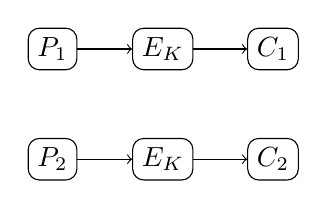
\begin{tikzpicture}[node distance=1.4cm]
    \node (p1) [draw, rounded corners] {$P_1$};
    \node (e1) [draw, rounded corners, right of=p1] {$E_K$};
    \node (c1) [draw, rounded corners, right of=e1] {$C_1$};
    \draw[->] (p1) -- (e1);
    \draw[->] (e1) -- (c1);
    \node (p2) [draw, rounded corners, below of=p1] {$P_2$};
    \node (e2) [draw, rounded corners, right of=p2] {$E_K$};
    \node (c2) [draw, rounded corners, right of=e2] {$C_2$};
    \draw[->] (p2) -- (e2);
    \draw[->] (e2) -- (c2);
  \end{tikzpicture}
  \caption{ECB: tiap blok independen.}
\end{figure}

\begin{figure}[htbp]
  \centering
  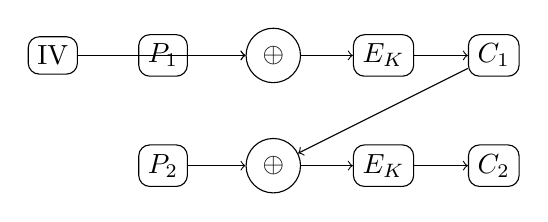
\begin{tikzpicture}[node distance=1.4cm]
    \node (iv) [draw, rounded corners] {IV};
    \node (p1) [draw, rounded corners, right of=iv] {$P_1$};
    \node (xor1) [draw, circle, right of=p1] {$\oplus$};
    \node (e1) [draw, rounded corners, right of=xor1] {$E_K$};
    \node (c1) [draw, rounded corners, right of=e1] {$C_1$};
    \node (p2) [draw, rounded corners, below of=p1] {$P_2$};
    \node (xor2) [draw, circle, right of=p2] {$\oplus$};
    \node (e2) [draw, rounded corners, right of=xor2] {$E_K$};
    \node (c2) [draw, rounded corners, right of=e2] {$C_2$};
    \draw[->] (iv) -- (xor1);
    \draw[->] (p1) -- (xor1);
    \draw[->] (xor1) -- (e1);
    \draw[->] (e1) -- (c1);
    \draw[->] (c1) -- (xor2);
    \draw[->] (p2) -- (xor2);
    \draw[->] (xor2) -- (e2);
    \draw[->] (e2) -- (c2);
  \end{tikzpicture}
  \caption{CBC: blok saling terikat melalui XOR.}
\end{figure}

\begin{figure}[htbp]
  \centering
  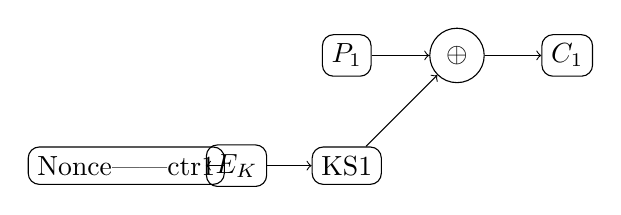
\begin{tikzpicture}[node distance=1.4cm]
    \node (n1) [draw, rounded corners] {Nonce||ctr1};
    \node (e1) [draw, rounded corners, right of=n1] {$E_K$};
    \node (k1) [draw, rounded corners, right of=e1] {KS1};
    \node (p1) [draw, rounded corners, above of=k1] {$P_1$};
    \node (xor1) [draw, circle, right of=p1] {$\oplus$};
    \node (c1) [draw, rounded corners, right of=xor1] {$C_1$};
    \draw[->] (n1) -- (e1);
    \draw[->] (e1) -- (k1);
    \draw[->] (p1) -- (xor1);
    \draw[->] (k1) -- (xor1);
    \draw[->] (xor1) -- (c1);
  \end{tikzpicture}
  \caption{CTR: keystream dari nonce||counter.}
\end{figure}

\subsection{Ringkasan Perbandingan Mode}

\begin{table}[htbp]
  \centering
  \small
  \begin{tabular}{lcccc}
    \toprule
    Mode & Perlu IV/Nonce & Perlu Padding & Paralel (enk) & Integritas \\
    \midrule
    ECB & Tidak & Ya & Ya & Tidak \\
    CBC & Ya & Ya & Tidak & Tidak \\
    CFB/OFB & Ya & Tidak & Sebagian & Tidak \\
    CTR & Ya & Tidak & Ya & Tidak \\
    GCM/CCM & Ya & Tidak & Ya & Ya \\
    \bottomrule
  \end{tabular}
  \caption{Perbandingan singkat mode operasi block cipher.}
\end{table}

\subsection{Contoh Pseudocode (CBC dan CTR)}

\begin{lstlisting}[style=cstyle, caption={CBC encryption (pseudocode)}]
for i = 0..n-1:
    x = P[i] ^ (i==0 ? IV : C[i-1]);
    C[i] = E_K(x);
\end{lstlisting}

\begin{lstlisting}[style=cstyle, caption={CTR encryption (pseudocode)}]
for i = 0..n-1:
    KS = E_K(nonce || counter);
    C[i] = P[i] ^ KS;
    counter++;
\end{lstlisting}

\begin{catatan}
Untuk keamanan, gunakan CBC, CFB, atau OFB dengan IV acak—bukan ECB. AES-CBC dan AES-GCM umum digunakan dalam praktik \cite{ferguson2010}.
\end{catatan}
